\documentclass[border=4pt]{standalone}
\usepackage{mathpazo}
\usepackage{xcolor}
\usepackage{tikz}
\usetikzlibrary{positioning,arrows.meta,fit,calc}
\definecolor{accent}{RGB}{96,96,32}
\begin{document}
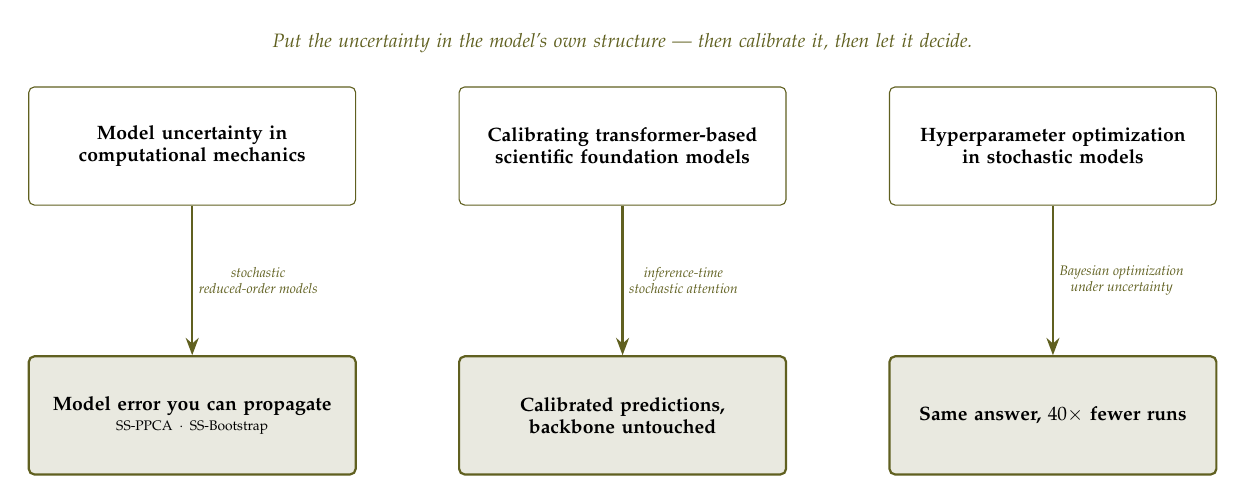
\begin{tikzpicture}[
  src/.style={draw=accent, rounded corners=2pt, align=center, font=\scriptsize,
              inner sep=5pt, text width=38mm, minimum height=15mm},
  res/.style={draw=accent, thick, fill=accent!14, rounded corners=2pt, align=center,
              font=\scriptsize, inner sep=5pt, text width=38mm, minimum height=15mm},
  arr/.style={-{Stealth[length=2.2mm]}, accent, thick},
  mid/.style={font=\tiny\itshape, text=accent, align=center, inner sep=2pt}]

\node[src] (a1) {\textbf{Model uncertainty in}\\\textbf{computational mechanics}};
\node[src, right=13mm of a1] (b1) {\textbf{Calibrating transformer-based}\\\textbf{scientific foundation models}};
\node[src, right=13mm of b1] (c1) {\textbf{Hyperparameter optimization}\\\textbf{in stochastic models}};

\node[res, below=19mm of a1] (a2) {\textbf{Model error you can propagate}\\[-1pt]{\tiny SS-PPCA $\cdot$ SS-Bootstrap}};
\node[res, below=19mm of b1] (b2) {\textbf{Calibrated predictions,}\\\textbf{backbone untouched}};
\node[res, below=19mm of c1] (c2) {\textbf{Same answer, $40\times$ fewer runs}};

\draw[arr] (a1) -- node[mid, right]{stochastic\\ reduced-order models} (a2);
\draw[arr] (b1) -- node[mid, right]{inference-time\\ stochastic attention} (b2);
\draw[arr] (c1) -- node[mid, right]{Bayesian optimization\\ under uncertainty} (c2);

\node[mid, above=3.5mm of b1, text width=105mm, font=\scriptsize\itshape]
  {Put the uncertainty in the model's own structure --- then calibrate it, then let it decide.};
\end{tikzpicture}
\end{document}
